\documentclass[conference]{IEEEtran}
\usepackage{cite}
\usepackage{amsmath,amssymb,amsfonts}
\usepackage{algorithmic}
\usepackage{graphicx}
\usepackage{textcomp}
\usepackage{xcolor}
\usepackage{url}
\def\BibTeX{{\rm B\kern-.05em{\sc i\kern-.025em b}\kern-.08em\TeX}}

\begin{document}

\title{Microarchitecture Simulation Assignment }

\author{\IEEEauthorblockN{Miguel Angel Alvarez Guzman}
\IEEEauthorblockA{
Estudiante Arquitectura Avanzada de Computadores \\
miguel.alvarezg@udea.edu.co}
}

\maketitle

\begin{abstract}

Este proyecto tiene como objetivo proporcionar a los lectores una visión integral sobre el análisis de un procesador ARM, al que se le modifican diversos parámetros para optimizar su rendimiento en la ejecución de programas específicos. Las pruebas se realizan en el entorno de simulación gem5, y el consumo de energía se evalúa utilizando la herramienta McPAT. A través de este estudio, se busca identificar las configuraciones óptimas del procesador que equilibran el rendimiento y la eficiencia energética.

\end{abstract}

\begin{IEEEkeywords}
Procesador ARM, Simulación gem5, Optimización de rendimiento, Consumo de energía, Herramienta McPAT, Configuración de parámetros, Arquitectura de computadores, Simulación de procesadores, Eficiencia energética, Análisis de rendimiento.
\end{IEEEkeywords}

\section{Introducción}
Este trabajo se ha realizado con el propósito de cumplir con los distintos objetivos de laboratorio propuestos por los profesores Sebastián Izasa y Luis Germán. En él se abordan diversas discusiones sobre los resultados obtenidos de las simulaciones, con el fin de mejorar el rendimiento predeterminado de un procesador ARM Cortex A76 utilizando los scripts proporcionados.

Se detallará la metodología empleada para seleccionar los parámetros a modificar y se analizará su impacto en el comportamiento global del procesador, incluyendo su consumo energético promedio. Además, se evaluará cómo estas modificaciones afectan el rendimiento de cada uno de los programas analizados, centrándose especialmente en el IPC (Instrucciones por Ciclo) y el Runtime Dynamic de cada caso.

\section{Metodología}

\subsection{Métodos}
\begin{itemize}
    \item \textbf{Configuración de gem5}:  
    La configuración inicial de gem5 se realizó revisando las diapositivas proporcionadas por los profesores y siguiendo las instrucciones para la correcta instalación y uso de gem5 y McPAT. Se realizaron prácticas con archivos de ejemplo disponibles tanto en la documentación de gem5 como en los scripts suministrados por los profesores. Además, se llevó a cabo una simulación inicial por defecto para cada uno de los seis programas entregados, con el objetivo de analizar el rendimiento base del procesador y determinar qué aspectos eran susceptibles de mejora.

    \item \textbf{Selección de Parámetros}:  
    Tras analizar los resultados de las simulaciones por defecto, se identificaron los parámetros críticos que requerían ajustes para optimizar el rendimiento del procesador. Los resultados iniciales mostraban:
    \begin{itemize}
        \item Alta cantidad de lecturas de memoria durante la ejecución.
        \item Alto uso de unidades ALU (Arithmetic Logic Unit) en operaciones de suma.
        \item Alta frecuencia de escrituras en memoria.
    \end{itemize}
    A partir de estas observaciones, se decidió modificar los siguientes parámetros para aumentar su capacidad o cantidad:
    \begin{itemize}
        \item Tamaño de la caché L2.
        \item Líneas de datos de la caché L2.
        \item Tamaño de la caché L3.
        \item Líneas de datos de la caché L3.
        \item Número de unidades funcionales para lectura de memoria.
        \item Número de unidades funcionales para las ALU enteras.
    \end{itemize}
    Se seleccionaron tres valores proporcionales para cada uno de estos parámetros, que fueron utilizados en las simulaciones para identificar las configuraciones óptimas.

    \item \textbf{Simulación}:  
    Para automatizar el proceso de simulación, se desarrolló un script que incorporaba todas las configuraciones posibles de los parámetros seleccionados. El script iteraba entre cada configuración y evaluaba los tres valores propuestos para cada parámetro, determinando el mejor de ellos en términos de rendimiento. Posteriormente, se usaba el valor óptimo de cada parámetro para realizar simulaciones adicionales sobre los otros parámetros.
\end{itemize}

\subsection{Técnicas}
\begin{itemize}
    \item \textbf{Análisis de Resultados por IPC}:  
    Al finalizar cada grupo de simulaciones, el script desarrollado en Python identificaba cuál era la configuración de parámetro que producía el mejor rendimiento para cada programa, utilizando como criterio principal el IPC (Instrucciones por Ciclo). Este enfoque permitía seleccionar la configuración más adecuada para optimizar el rendimiento en cada etapa de simulación.

    \item \textbf{Optimización Iterativa}:  
    La técnica de optimización iterativa se utilizó para ajustar cada parámetro de manera secuencial, fijando los valores óptimos obtenidos en cada paso antes de pasar a la evaluación del siguiente parámetro. Este proceso aseguraba que los cambios realizados en un parámetro no se vean afectados negativamente por las modificaciones en otros.
\end{itemize}

\subsection{Herramientas}
\begin{itemize}
    \item \textbf{gem5}:  
    gem5 fue utilizado como la plataforma de simulación para modelar el comportamiento del procesador ARM Cortex A76 y analizar el impacto de diferentes configuraciones de parámetros sobre su rendimiento.

    \item \textbf{McPAT}:  
    McPAT se empleó para evaluar el consumo energético de cada configuración simulada en gem5. Al finalizar cada simulación, se generaban los resultados de rendimiento, que luego se pasaban a McPAT para calcular el consumo energético, incluyendo el Runtime Dynamic y otros indicadores relevantes.

    \item \textbf{Python}:  
    Se utilizó Python para desarrollar un script que automatizaba la gestión de las simulaciones y el análisis de resultados. El script controlaba las iteraciones de configuración de parámetros y seleccionaba los valores óptimos según el IPC de cada simulación, permitiendo un proceso más eficiente y menos propenso a errores.
\end{itemize}

\section{Resultados}

\subsection{Resultados de Perfiles}

\begin{figure}[htbp]
\centering
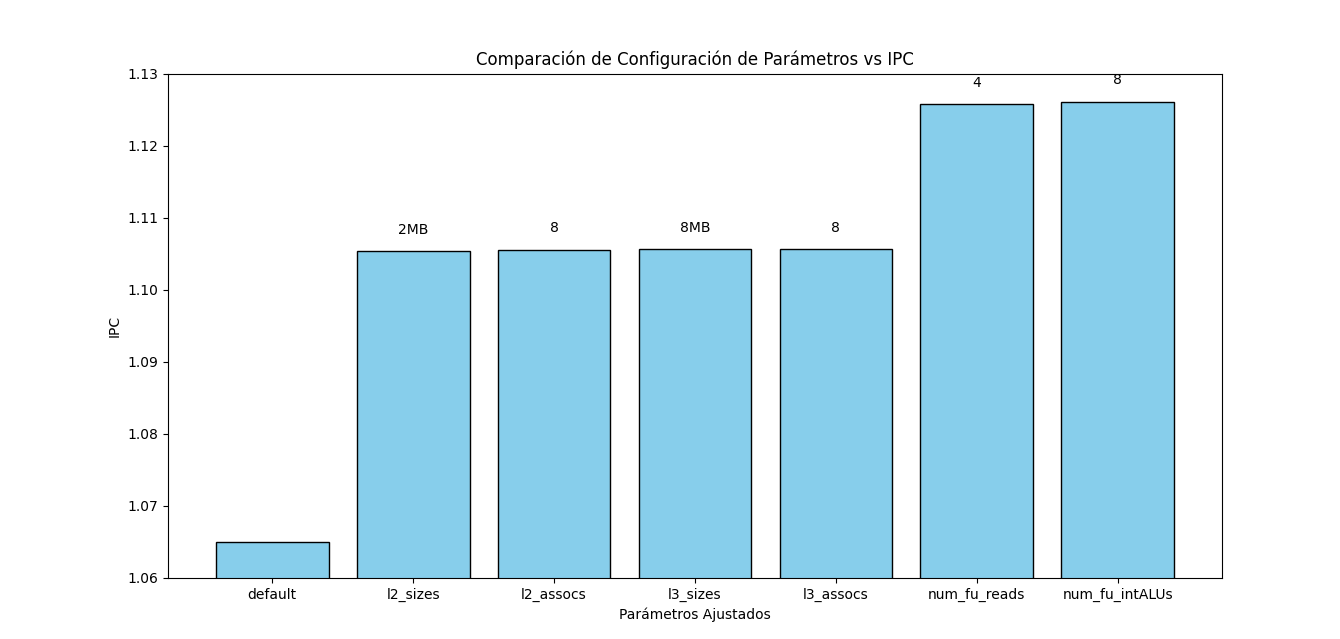
\includegraphics[width=0.5\textwidth]{Barras_IPC_1.png}
\caption{Resultados h264 dec en funcion de los mejores parametros cambiados}
\label{fig:example}
\end{figure}

\begin{figure}[htbp]
\centering
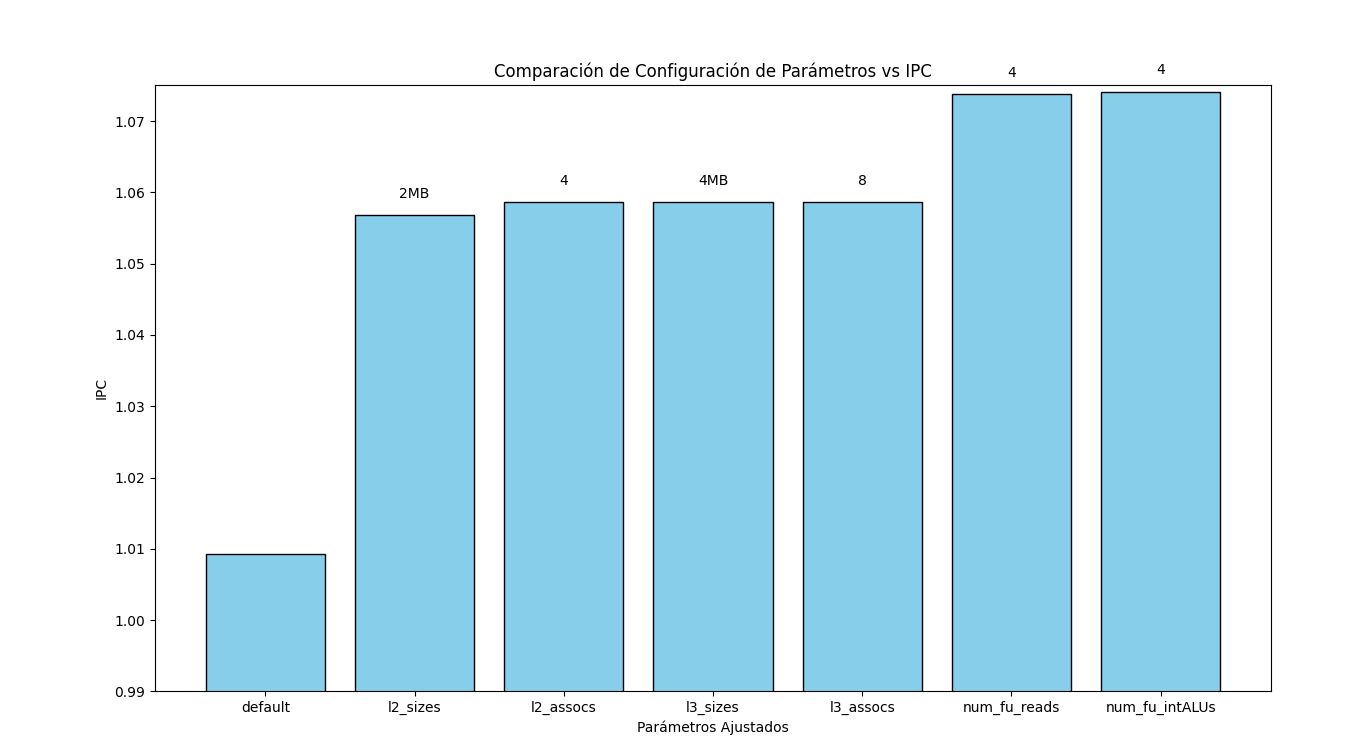
\includegraphics[width=0.5\textwidth]{Barras_IPC_2.png}
\caption{Resultados h264 enc en funcion de los mejores parametros cambiados}
\label{fig:example}
\end{figure}
\newpage
\begin{figure}[htbp]
\centering
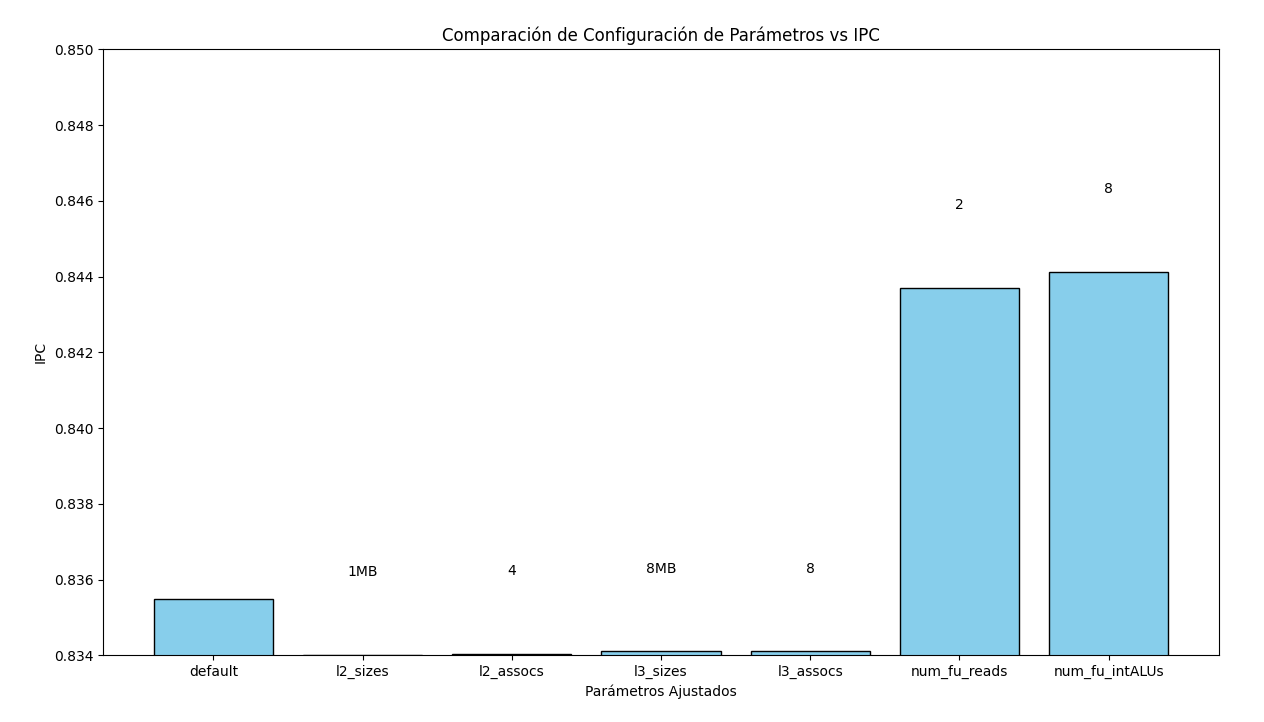
\includegraphics[width=0.5\textwidth]{Barras_IPC_3.png}
\caption{Resultados jpg2k dec en funcion de los mejores parametros cambiados}
\label{fig:example}
\end{figure}
\begin{figure}[htbp]
\centering
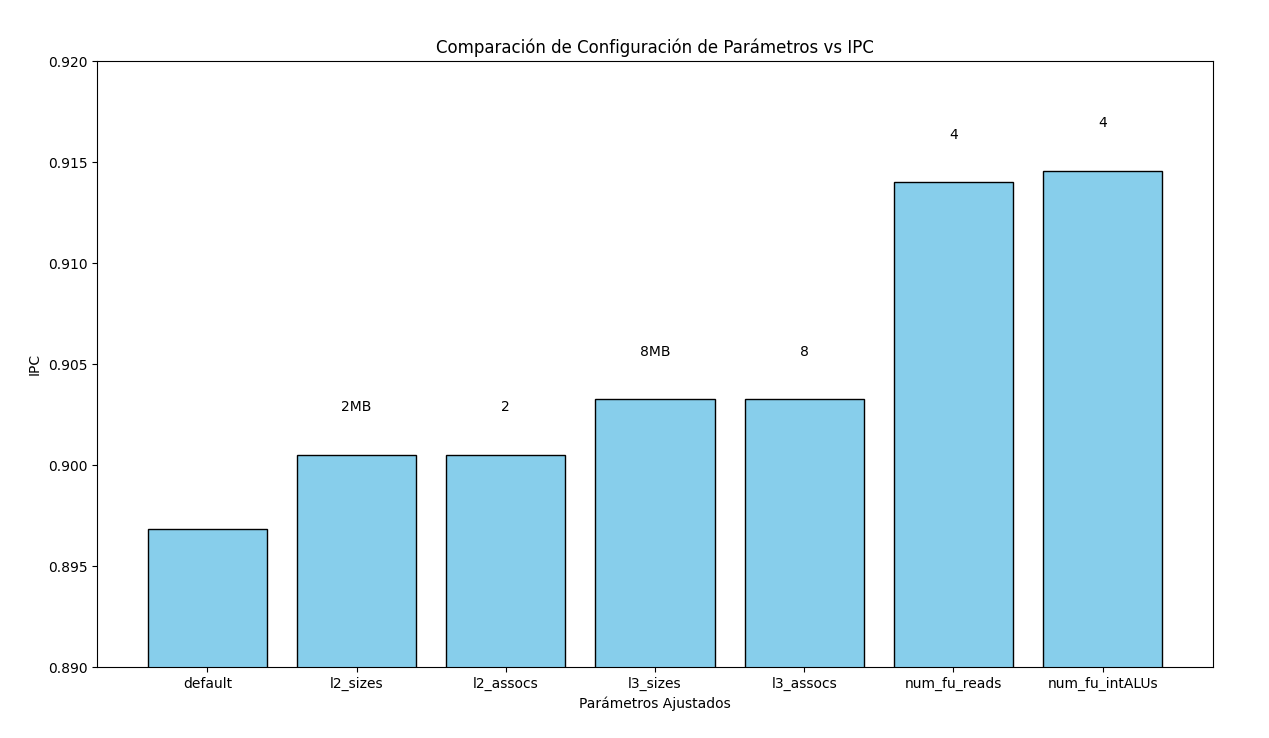
\includegraphics[width=0.5\textwidth]{Barras_IPC_4.png}
\caption{Resultados jpg2k enc en funcion de los mejores parametros cambiados}
\label{fig:example}
\end{figure}
\begin{figure}[htbp]
\centering
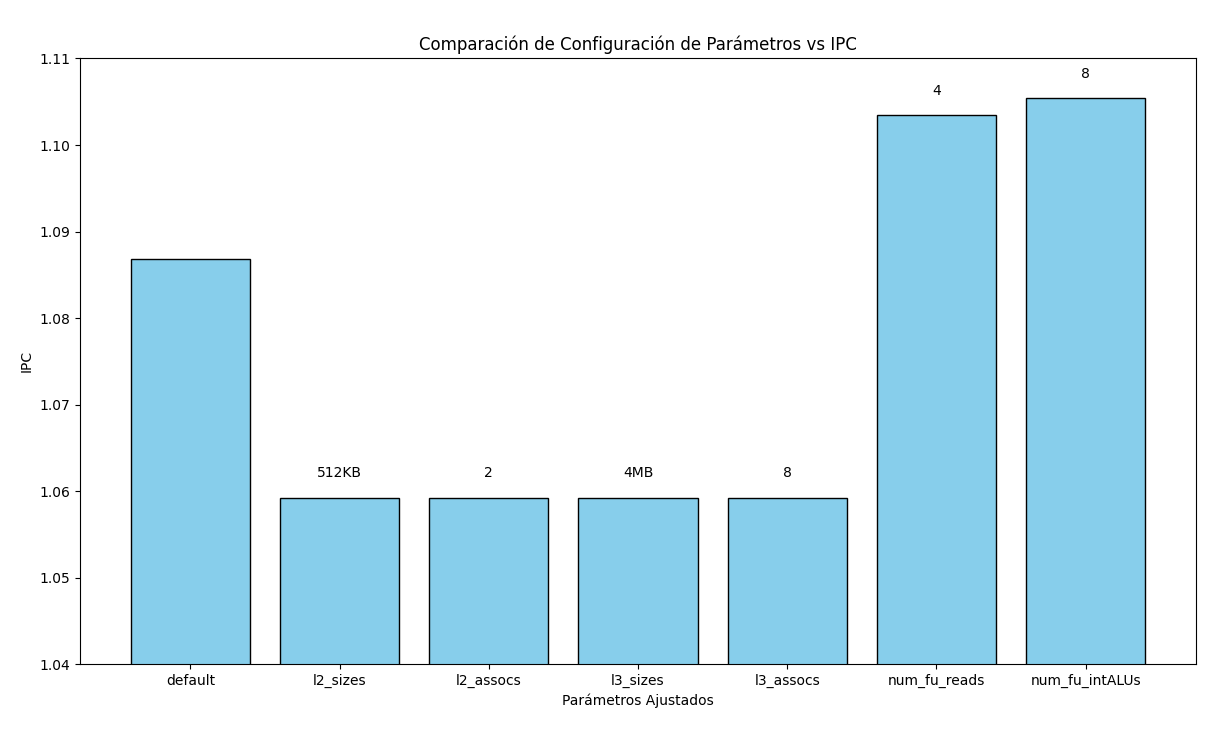
\includegraphics[width=0.5\textwidth]{Barras_IPC_5.png}
\caption{Resultados mp3 dec en funcion de los mejores parametros cambiados}
\label{fig:example}
\end{figure}
\newpage
\begin{figure}[htbp]
\centering
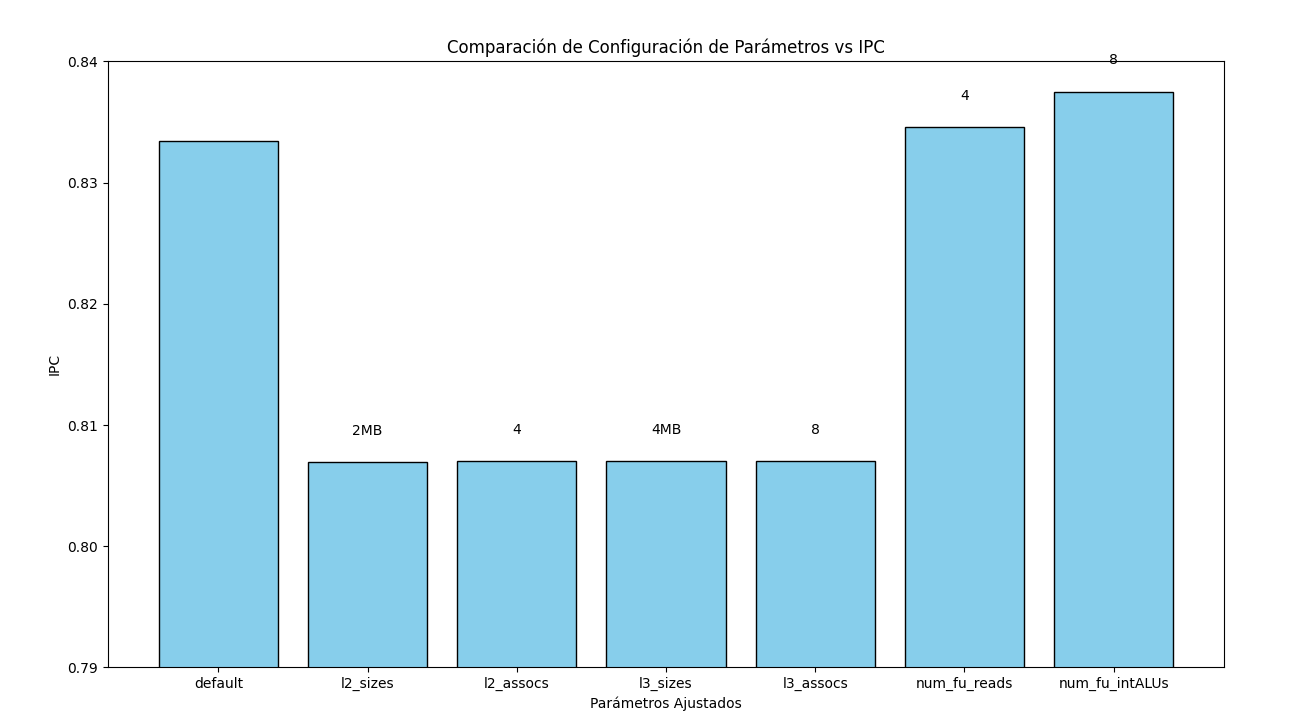
\includegraphics[width=0.5\textwidth]{Barras_IPC_6.png}
\caption{Resultados mp3 enc en funcion de los mejores parametros cambiados}
\label{fig:example}
\end{figure}

\subsection{Rendimiento contra recursos}
\begin{figure}[htbp]
\centering
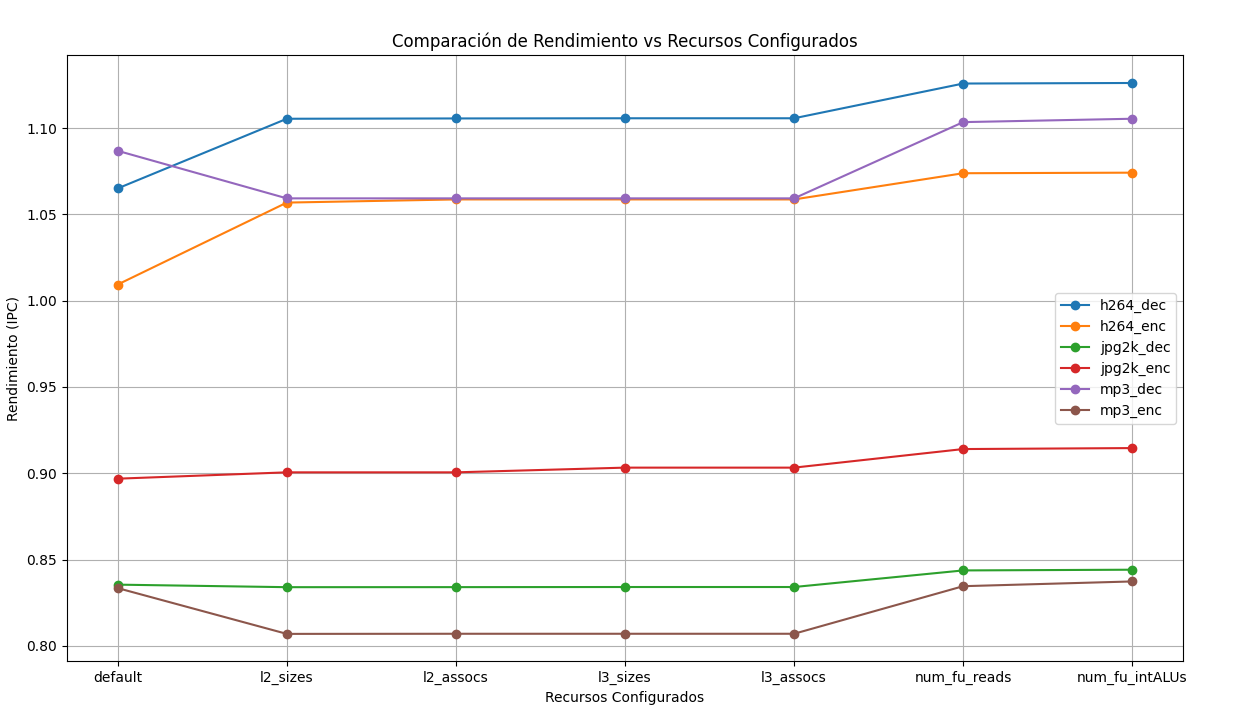
\includegraphics[width=0.5\textwidth]{Lineas_IPC.png}
\caption{Resultados de los programas en funcion de los recursos usados}
\label{fig:example}
\end{figure}

\subsection{Grafico de rendimiento contra energia}
\begin{figure}[htbp]
\centering
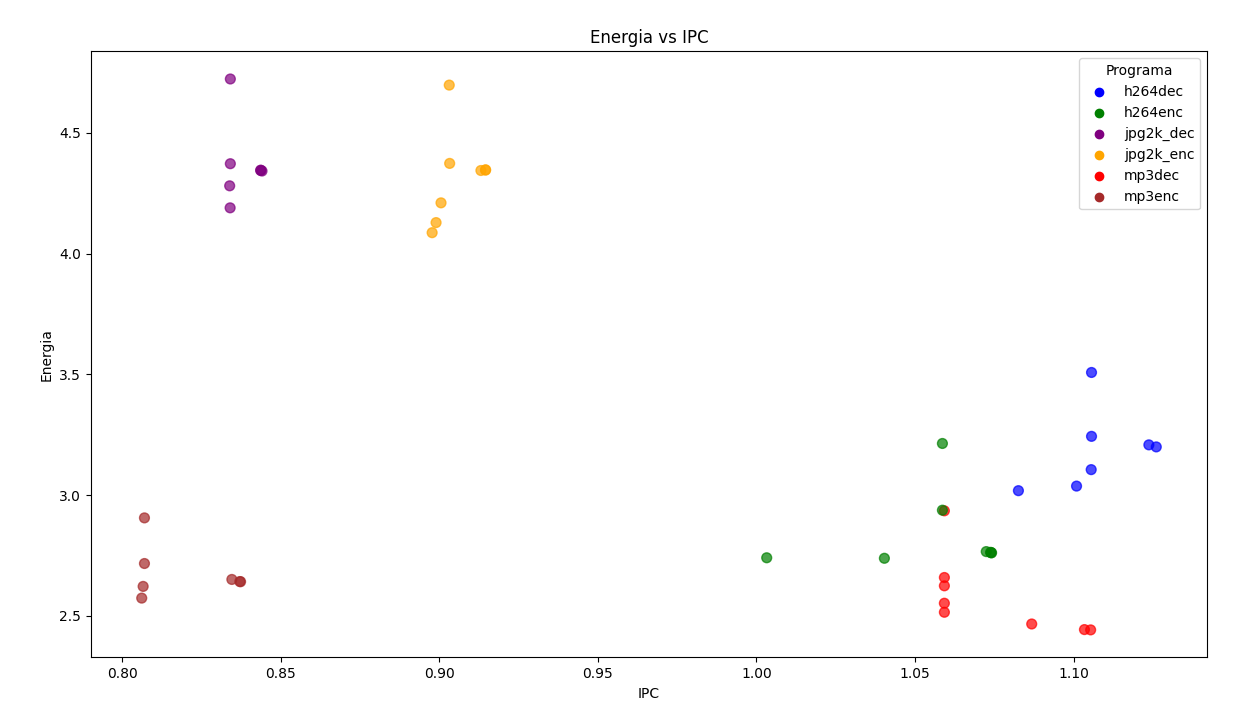
\includegraphics[width=0.5\textwidth]{Plotter_IPC_Energy.png}
\caption{Comparacion de la energia usada contra el IPC generado por programa.}
\label{fig:example}
\end{figure}
\newpage
\subsection{Mejores Rendimientos}
\begin{figure}[htbp]
\centering
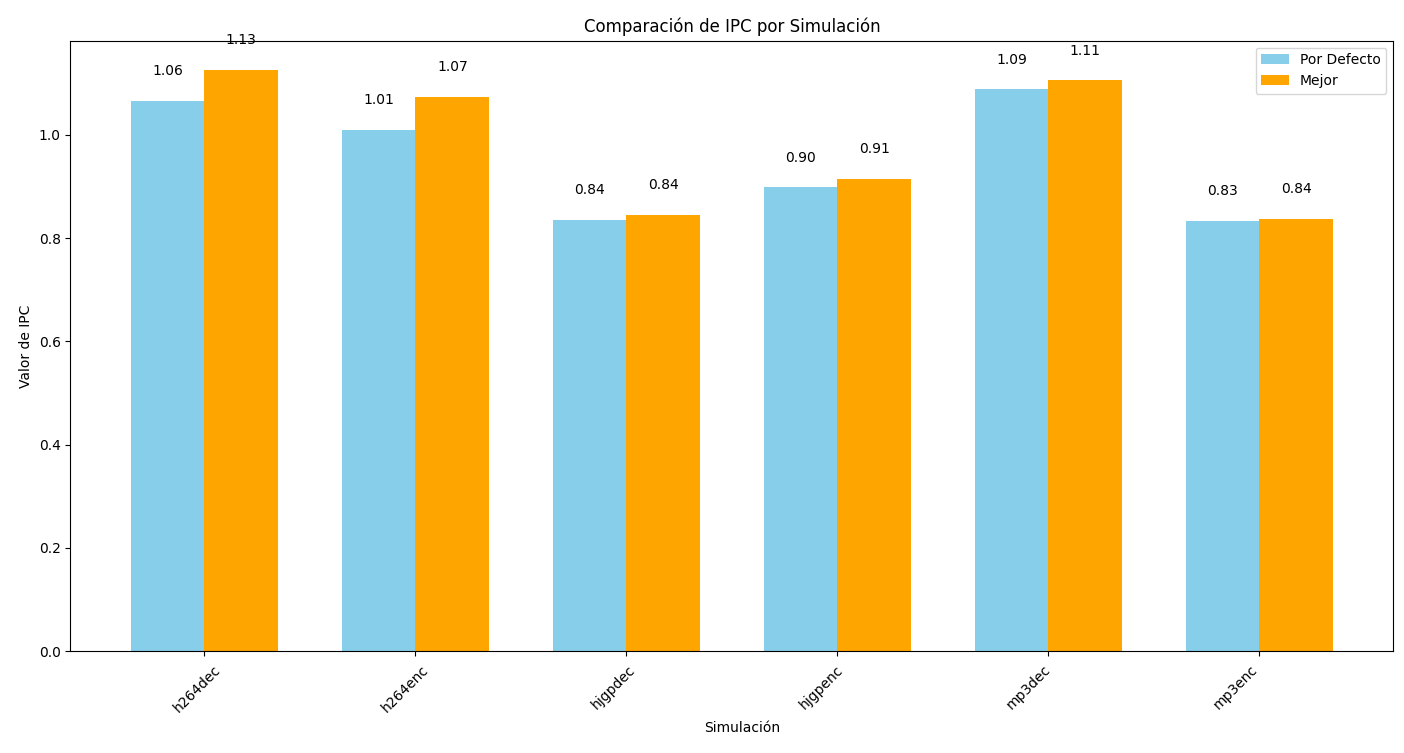
\includegraphics[width=0.5\textwidth]{Mejor_IPC.png}
\caption{Grafica de Mejor IPC por simulacion}
\label{fig:example}
\end{figure}

\begin{figure}[htbp]
\centering
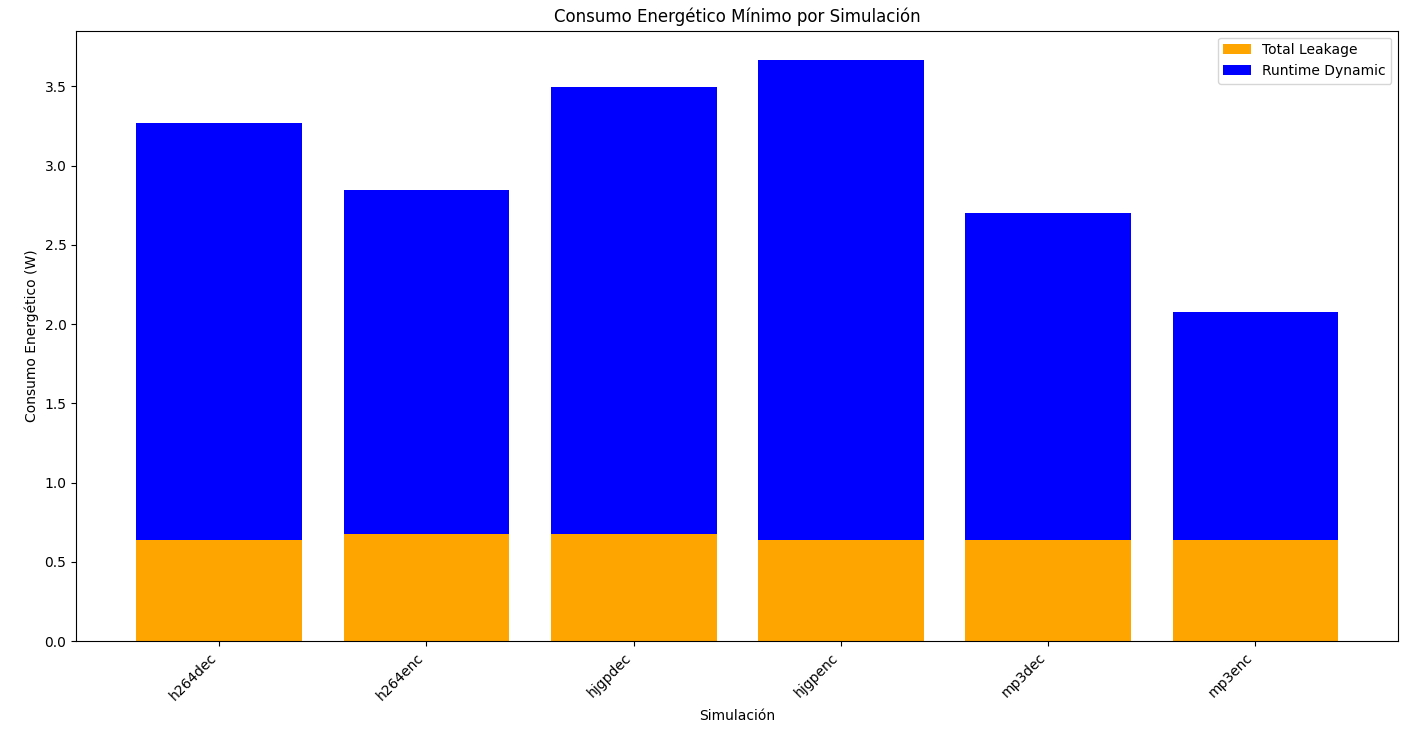
\includegraphics[width=0.5\textwidth]{Mejor_Energia.png}
\caption{Grafica de menor consumo por simulacion}
\label{fig:example}
\end{figure}

\begin{figure}[htbp]
\centering
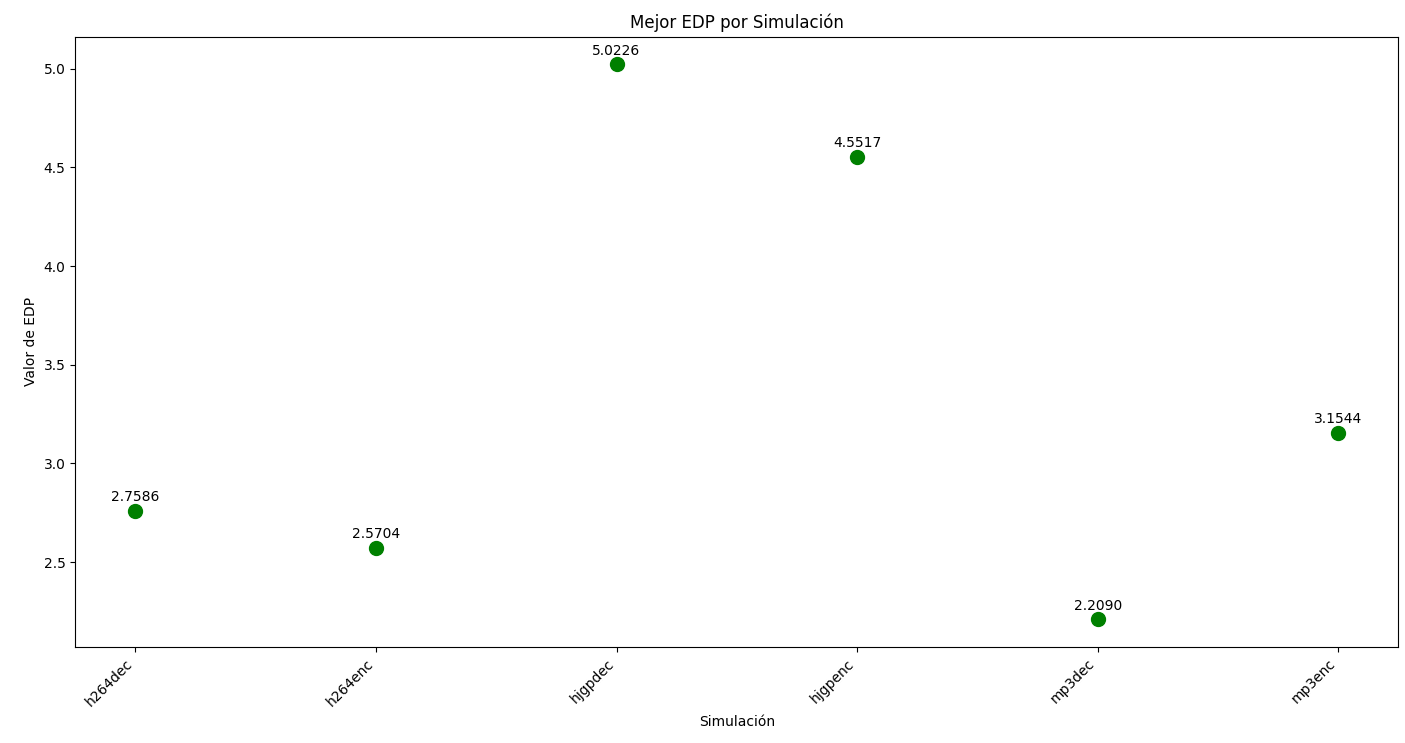
\includegraphics[width=0.5\textwidth]{Mejor_EDP.png}
\caption{Grafica de mejor EDP por simulacion}
\label{fig:example}
\end{figure}
\newpage
\subsection{Tiempo de Ejecucion}
\begin{figure}[htbp]
\centering
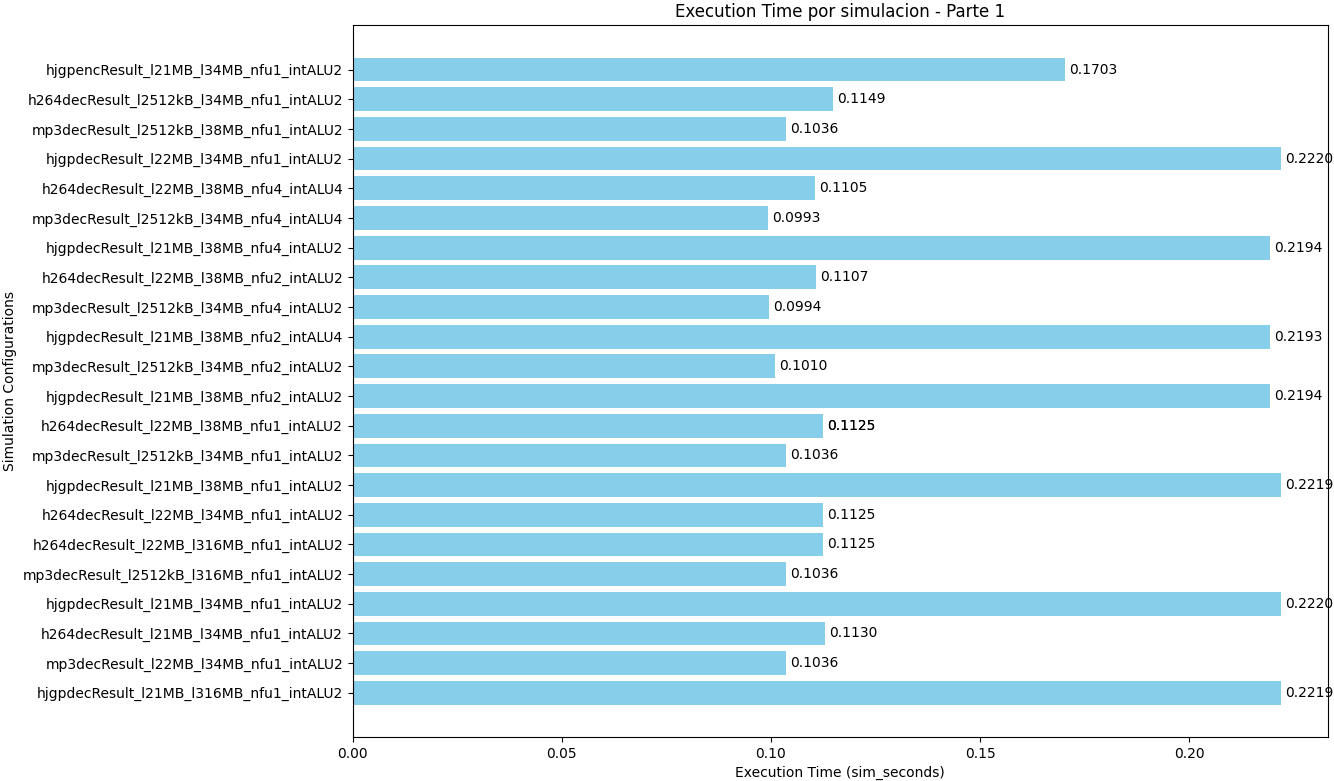
\includegraphics[width=0.5\textwidth]{Tiempo_Ejecucion_1.png}
\caption{Grafica de Tiempo de ejecucion por simulacion 1}
\label{fig:example}
\end{figure}
\subsection{Tiempo de Ejecucion}
\begin{figure}[htbp]
\centering
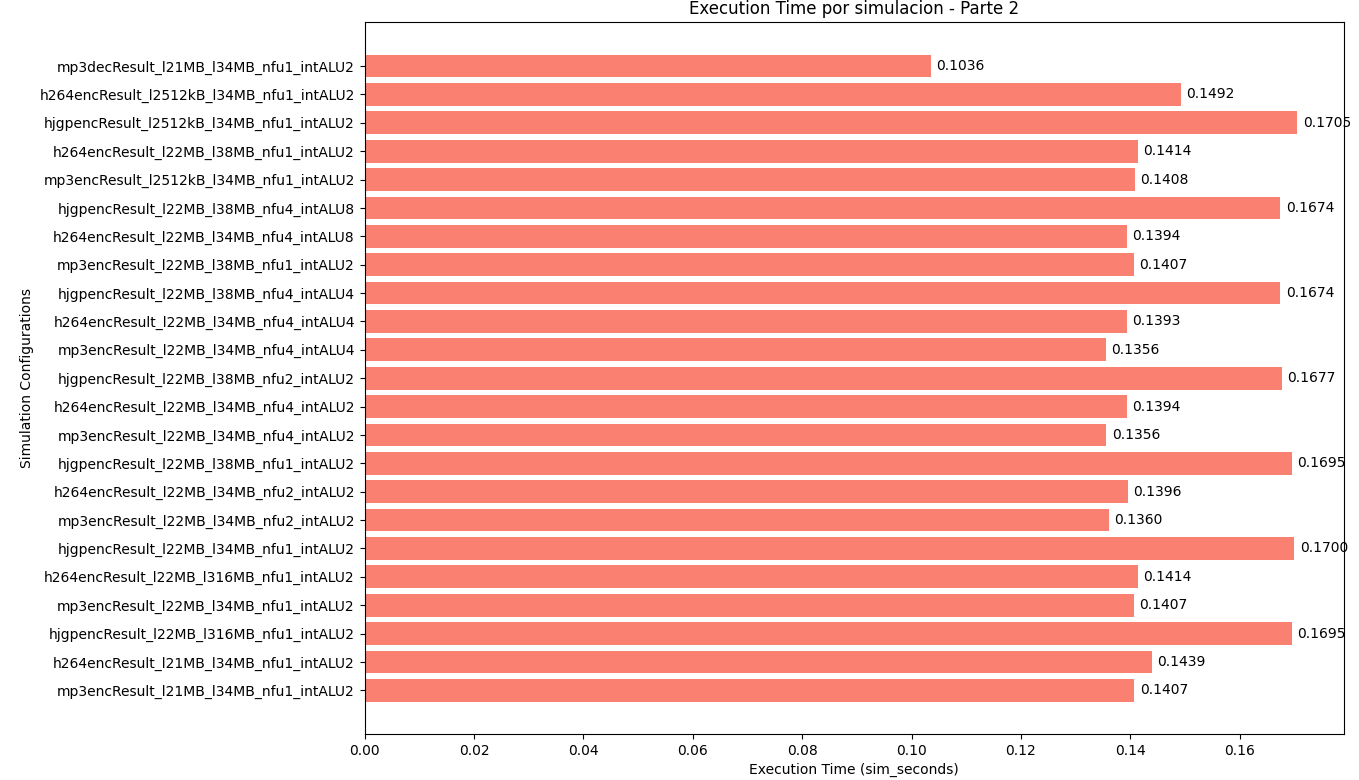
\includegraphics[width=0.5\textwidth]{Tiempo_Ejecucion_2.png}
\caption{Grafica de Tiempo de ejecucion por simulacion 2}
\label{fig:example}
\end{figure}
\newpage
\section{Discusión}

\subsection{Análisis de Resultados por Perfiles}

Los resultados obtenidos para cada simulación muestran las configuraciones óptimas derivadas de la modificación de tres parámetros principales en cada programa. Estos parámetros fueron ajustados iterativamente para maximizar el rendimiento, representado principalmente por el IPC (Instrucciones por Ciclo). A continuación, se presenta una discusión detallada de los resultados obtenidos para cada simulación.

\subsubsection{Simulación h264 dec}

En la simulación de decodificación h264, se observó un aumento considerable en el IPC en comparación con la configuración por defecto. Este incremento se atribuye principalmente al aumento en el número de unidades funcionales de lectura y al tamaño de la caché L2. Los demás parámetros mostraron una influencia mínima en la mejora del IPC, sugiriendo que la lectura de memoria y el acceso rápido a la caché fueron determinantes en este contexto.

\subsubsection{Simulación h264 enc}

Para la simulación de codificación h264, el rendimiento se vio significativamente mejorado al incrementar el tamaño de la caché L2 y el número de unidades de lectura de memoria. Aunque la adición de líneas de datos en la caché L2 también contribuyó, su impacto fue menor. Los otros parámetros evaluados mostraron variaciones mínimas respecto al rendimiento, indicando que los ajustes en la caché y las unidades de lectura de memoria son cruciales para este programa.

\subsubsection{Simulación jpg2k dec}

En la decodificación jpg2k, aumentar el tamaño de la caché L2 resultó en una disminución en el rendimiento, mostrando un IPC más bajo que en la configuración inicial. No obstante, una leve mejora en el IPC se logró al ajustar otros parámetros, especialmente al incrementar las unidades de lectura y las unidades funcionales ALU. Esto sugiere que el procesamiento ALU es crítico para el rendimiento en este caso.

\subsubsection{Simulación jpg2k enc}

La codificación jpg2k mostró mejoras constantes sobre la configuración predeterminada, con incrementos de rendimiento evidentes al aumentar los tamaños de caché L2 y L3 y al incrementar tanto las unidades funcionales de lectura como las ALU. Estos resultados sugieren que las configuraciones de caché y las unidades funcionales juegan un papel importante en la eficiencia del procesamiento de este programa.

\subsubsection{Simulación mp3 dec}

En la simulación de decodificación mp3, el rendimiento disminuyó en la mayoría de las configuraciones en comparación con la configuración por defecto, excepto cuando se aumentaron las unidades funcionales de lectura y las ALU. Estos ajustes lograron mitigar la caída en el rendimiento, destacando nuevamente la importancia de las unidades funcionales para ciertos tipos de procesamiento.

\subsubsection{Simulación mp3 enc}

Para la codificación mp3, el único cambio que resultó en una mejora ligera fue el aumento de las unidades funcionales de lectura y ALU. En todas las demás configuraciones, se observó una disminución en el rendimiento, lo cual indica que estos recursos específicos son necesarios para optimizar este tipo de carga de trabajo.

\subsection{Análisis de Rendimiento contra Recursos}

La gráfica de rendimiento ponderado en función de los recursos utilizados muestra cómo la variación de cada parámetro afecta el IPC. En general, aumentar las líneas de datos en las cachés L2 y L3 tuvo un impacto prácticamente insignificante en el rendimiento final. En cambio, aumentar el número de unidades funcionales de lectura resultó en mejoras significativas en todos los programas. Esto sugiere que no todos los aumentos de recursos se traducen en mejoras en el rendimiento, e incluso, en dos casos, provocaron una disminución.

\subsection{Análisis de Rendimiento contra Energía}

La comparación gráfica entre el consumo de energía y el IPC muestra que, en términos generales, las simulaciones basadas en un mismo programa mantienen una variabilidad de consumo energético bastante estrecha, con una dispersión de aproximadamente ±1 W. Esto sugiere una relativa estabilidad en el consumo energético al variar los parámetros, lo cual es útil para predecir el rendimiento energético en configuraciones similares.

\subsection{Análisis de Mejores Rendimientos}

Las gráficas que presentan los valores óptimos alcanzados en cada simulación reflejan las mejores configuraciones de parámetros específicas, documentadas en un archivo de Resultados Óptimos disponible en el repositorio de GitHub. Estos valores indican las configuraciones más efectivas en cuanto a rendimiento (IPC), consumo mínimo y eficiencia energética (EDP), detallados a continuación:

\subsubsection{Mejor IPC por Simulación}

Esta gráfica muestra los valores de IPC óptimos para cada programa, destacando las mejoras alcanzadas en comparación con las configuraciones por defecto. Se observa una mejora en el IPC en todos los programas, siendo particularmente notable en las simulaciones de codificación y decodificación h264.

\subsubsection{Menor Consumo por Simulación}

Los resultados en la gráfica de menor consumo energético resaltan las configuraciones que presentaron el consumo más bajo en cada simulación. Estas optimizaciones permiten identificar las configuraciones menos demandantes de energía en cada caso de prueba.

\subsubsection{Mejor EDP por Simulación}

Según los resultados, al evaluar el rendimiento en función del EDP (Energy Delay Product), se destaca la decodificación jpg2k como la que logra el mayor EDP, evidenciando que este parámetro proporciona una perspectiva útil para balancear la eficiencia energética y el rendimiento.

\subsection{Análisis del Tiempo de Ejecución}

Las gráficas de tiempo de ejecución ilustran cómo se distribuyó el tiempo en cada simulación en función de los parámetros ajustados. A medida que se optimizan los parámetros, el tiempo de ejecución tiende a disminuir, lo que indica mejoras en el rendimiento global de las simulaciones.

\section{Conclusiones}

Los resultados de este estudio permiten extraer varias conclusiones importantes sobre el impacto de la modificación de parámetros en el rendimiento y la eficiencia energética de un procesador ARM en simulaciones específicas. A continuación, se resumen los hallazgos clave:

Impacto de las Unidades Funcionales: En la mayoría de los programas analizados, el aumento en el número de unidades funcionales de lectura y ALU mostró una mejora considerable en el rendimiento, especialmente en términos de IPC. Esto indica que, para optimizar tareas que requieren alto acceso a la memoria y procesamiento aritmético, la disponibilidad de unidades funcionales adicionales es un factor clave.

Limitaciones de los Aumentos en la Caché: Los incrementos en el tamaño y las líneas de datos de las cachés L2 y L3 no siempre resultaron en mejoras significativas en el rendimiento. En algunos casos, como en las simulaciones de jpg2k dec y mp3 enc, incluso se observó una disminución en el IPC. Esto sugiere que un aumento de caché no necesariamente implica un mejor desempeño, y que la efectividad de la caché depende de la naturaleza específica de las tareas.

Balance entre Consumo Energético y Rendimiento: Las gráficas de rendimiento contra energía muestran que es posible lograr mejoras en el IPC sin un incremento proporcional en el consumo energético. Este hallazgo es relevante para aplicaciones que requieren un balance entre eficiencia y rendimiento, ya que demuestra que es posible optimizar el procesador sin penalizar significativamente el consumo de energía.

Eficiencia Energética con EDP: El análisis del EDP (Energy Delay Product) reveló que ciertas configuraciones lograron un equilibrio óptimo entre el tiempo de ejecución y el consumo energético. Esto se observó particularmente en la decodificación de jpg2k, donde los ajustes lograron maximizar el EDP. Este parámetro es fundamental para seleccionar configuraciones que ofrezcan rendimiento con un consumo energético moderado.

Optimización Iterativa de Parámetros: La metodología de optimización iterativa utilizada en este estudio demostró ser efectiva para mejorar el rendimiento sin comprometer el análisis de las interacciones entre parámetros. La técnica asegura que los ajustes de un parámetro no afecten de forma adversa los cambios de otros, permitiendo un proceso de optimización más preciso.

Adaptabilidad de las Configuraciones: Los resultados sugieren que no existe una configuración única que maximice el rendimiento en todas las simulaciones; más bien, las configuraciones óptimas son específicas a cada tipo de programa. Esto implica que las estrategias de optimización deben adaptarse a la carga de trabajo específica para obtener el mejor balance entre rendimiento y eficiencia energética.

En conclusión, este estudio aporta un marco sólido para la selección de configuraciones de procesadores ARM, mostrando que el ajuste selectivo de parámetros como las unidades funcionales y la caché puede mejorar significativamente el rendimiento en simulaciones específicas. A futuro, se recomienda realizar pruebas adicionales con diferentes arquitecturas y tipos de aplicaciones para generalizar estos hallazgos y validar la metodología de optimización en otros contextos.

\section{Referencias}

[1] Proyecto y código fuente disponible en: \url{https://github.com/jbcgames/General_Test}.

\end{document}
